\chapter{Desarrollo del Proyecto}

\minitoc

\section{Introducción}

\begin{figure}[!tb]
	\centering
	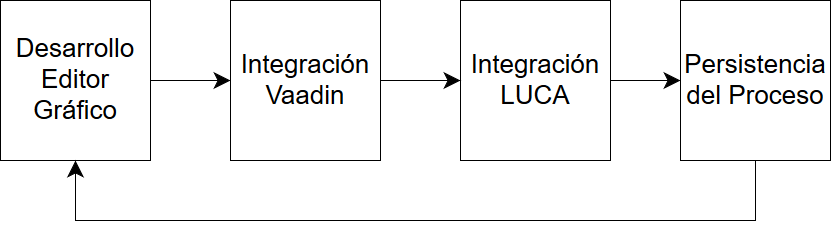
\includegraphics[width=\linewidth]{flujoDesarrollo.png}
	\caption{Flujo de Desarrollo}
	\label{fig:flujoDesarrollo}
\end{figure}

%% Decir qué cuenta esta sección y los pasos generales que se han dado para
%% desarrollar el \emph{Process Editor}

El presente capítulo detalla el proceso de desarrollo del proyecto realizado dentro de este Trabajo Fin de Grado. Tal como se ha comentado, el objetivo del proyecto era 
proporciona al producto LUCA una herramienta gráfica para poder crear \emph{procesos}, es decir, poder encadenar consultas entre sí a raíz de sus valores de entrada y de salida.

Para alcanzar este objetivo, se siguió el esquema de trabajo que se muestra en la Figura~\ref{fig:flujoDesarrollo}.  

La primera etapa consistió en realizar un primer contacto con la herramienta \emph{GoJS}, para ello, se realizó una prueba de concepto donde se creaba un diagrama sencillo con cajas o nodos que se conectan entre sí (Figura~\ref{}).

Con la prueba de concepto funcionando, la siguiente etapa consistió en integrar el diagrama en \emph{GoJS} con el framework de \emph{Vaadin} para obtener un proyecto implementado en \emph{Java} que pueda ser utilizado por otro proyectos, es decir, crear un proyecto que actúa de herramienta gráfica de forma genérica a cualquier otro proyecto que le quiera utilizar.

La tercera etapa se centró en integrar dicho proyecto \emph{Vaadin}, antes mencionado, en el producto LUCA con el objetivo de ser capaces de mostrar el editor y ser capaces de interactuar con él y recibir los eventos ocurridos.

Por último, la cuarta etapa consistió en añadir la capa de negocio y de persistencia al modelo de datos de LUCA, creado específicamente para persistir \emph{procesos} y toda su jerarquía de clases.

Una vez acabadas las cuatro etapas de desarrollo, comenzó un curso de iteraciones para refinar el proyecto e ir dando la complejidad final al mismo, de forma que se fue completando toda la lógica de negocio, así como, el aspecto gráfico final.

Las siguientes secciones proporcionan detalles sobre la ejecución de cada etapa.

\section{Desarrollo del Editor Gráfico}

%% Describir los pasos, a nivel general, para crear el editor gráfico sencillo. 
El editor gráfico utiliza \emph{GoJS} para crear toda la interfaz visual, este framework (como ya se explicó en el apartado de documentación) utiliza \emph{templates} para definir el aspecto estético de los diferentes componentes. Por lo tanto, el primer paso tras tener claro cómo debía de ser un primer boceto de interfaz fue crear todos los \emph{templates} de los que se iba a componer.

El segundo paso, una vez conseguida la estética y estructura de elementos deseada, fue comprobar la funcionalidad del mismo, desde asegurar que al interactuar con el editor se creaban los eventos oportunos, hasta comprobar que los elementos se mostraban en pantalla tal y como se quería.

%% Añadir algo de código. 


%% Qué se hizo en otras iteraciones, a modo de la lista de la compra (y teniendo en 
%%    cuenta que son cosas gráficas)
Con la primera prueba de concepto terminada, las siguientes iteraciones se centraron en otorgar nuevas funcionalidades al diseño:
\begin{itemize}
	\item Permitir cambiar colores y tamaños de los elementos desde el exterior, es decir, desde una aplicación que utilice esta herramienta o gráfico.
	\item Permitir crear elementos con diferentes formas a partir de formas prediseñadas en \emph{GoJS} o a partir de imágenes \emph{SVG}\cite{svg}.
\end{itemize}

%% Código de aquello en lo que te quieras lucir (opcional)
Durante el proceso gráfico de enlazado de elementos, fue necesaria la modificación de la operación de enlazar. Por defecto, cuando se crea un enlace entre dos elementos, se crea un evento de enlazado y además, se añade al modelo de datos de \emph{GoJS} un \emph{link} entre los dos elementos. Debido a la lógica que se deseaba conseguir, en el flujo de creación de un enlace, \emph{GoJS} solo se tiene de encargar en una primera instancia de enviar el evento de enlazado, y después cuando se le comunique, crear gráficamente dicho enlace, sin embargo, como ya se ha dicho, por defecto se crea el enlace y se manda un evento que comunica su creación. Para conseguir la funcionalidad deseada, hubo que modificar la herramienta de enlazado (\emph{LinkTool}, es la encargada de producir eventos y modificar el modelo durante el proceso de enlazado) para que enviase el evento exclusivamente.
%% Hablar algo de pruebas. 
Debido a que esta herramienta se focaliza en representar información sobre una interfaz, se prescindió la creación de pruebas automatizadas debido a su complejidad e inversión de tiempo. 

\section{Integración del editor con \emph{Vaadin}}

%% Explicar que necesitamos hacer que los eventos del editor se redirijan a Vaadin
El objetivo principal del editor gráfico de \emph{procesos} es proporcionar una interfaz, con la que otros proyectos que quieran utilizar este editor se puedan comunicar para poder gestionar los \emph{procesos}.

%% Explicar que la redirección se hace mediante un conector en Javascript
Para ello es necesario que exista una comunicación entre la herramienta \emph{GoJS} y \emph{Vaadin} mediante eventos. Estos eventos producidos en \emph{GoJS} son trasladados al proyecto \emph{Vaadin}, para que sean comunicados al proyecto que utilice este componente gráfico (en nuestro caso, este papel lo ocupara el producto de LUCA, que deberá decidir que eventos escuchar y como reaccionar ante ellos).

Para que esta comunicación entre \emph{GoJS} y \emph{Vaadin} sea posible, es necesario un fichero que realice las funciones de conector (a partir de ahora lo llamaremos \emph{conector}), su objetivo será comunicar a \emph{Vaadin} de los eventos ocurrido en el editor gráfico y, siguiendo las órdenes de \emph{Vaadin} realizar cambios sobre la interfaz del editor gráfico. De esta forma se produce un diálogo entre ambos conceptos en base a eventos y cambios en la interfaz gráfica.


%% Mostrar un trozo de código del conector muy sencillo

%% Explicar que en algunos casos fue necesario alterar el flujo de funcionamiento 
%% normal de GoJS y describir el caso del link.
En algunas ocasiones fue necesaria  modificar el comportamiento interno de algunas funciones de \emph{GoJS}, por ejemplo, cuando se realiza una conexión a nivel gráfico, en el modelo de \emph{GoJS} se instancia un enlace, sin embargo, debido a que no se requería de dicha funcional (sino que lo que se quería era solo mandar el evento de enlazado, para después, si era necesario enlazar), fue necesario sobreescribir dicha funcionalidad para evitar que se produzca dicha instanciación (Figura~\ref{}).

%% Explicar figura del link

%% Hablar algo de pruebas. 
Debido a la complejidad que existe para comprobar que las acciones que se realizan desde el proyecto del editor a nivel \emph{Java} se muestran gráficamente en el editor, no se han realizado pruebas automatizadas, aunque si se realizaron pruebas o verificaciones del funcionamiento visualmente en base a las acciones que se pueden realizar sobre el mismo, como son la creación de procesos y enlazado entre ellos.


\section{Integración del editor con LUCA}

%% Decribir los pasos, a nivel general, para integrar el editor básico. 
Como el editor gráfico actúa como un componente propio de \emph{Vaadin}, para integrarlo en un proyecto (en nuestro caso LUCA) es tan simple como incluirlo en una vista (utilizando el ya explicado patrón \emph{Mode-View-Presenter}). Una vez que la vista ya alberga dicho componente (a partir de ahora lo llamaremos \emph{DiagramComponent}), es necesario al crear el presentador, crear una instancia del mismo. De esta forma el componente ya está preparado para ser utilizado y mostrar el diagrama. Por último sería necesario mandar las directrices de creación de un proceso y/o subprocesos, es decir, consultas que queremos utilizar, para que sean dibujadas en el editor.
%% Mostrar captura de la interfaz

%% Qué se hizo en otras iteraciones, a modo de la lista de la compra.
En las siguientes iteraciones en esta etapa, se creó la vista de gestión para la creación, edición y eliminado de procesos, la vista de gestión de procesos que pueden ser ejecutados, y una nueva vista para ejecutar un proceso. Además se enriqueció la vista de gestión creada inicialmente para construir un proceso utilizando el editor gráfico.
%% Mostrar código de algo no trivial 

%% Hablar algo de pruebas. 
Las pruebas que se realizaron sobre esta etapa consistieron en el envío y recepción de los eventos que se producen entre el editor gráfico y LUCA. Sin embargo, no se realizó un automatización del las pruebas debido a la complejidad y tiempo necesario que requería.

\section{Gestión y Persistencia de los Procesos}

El objetivo de este paso era que LUCA pudiese almacenar y gestionar procesos. Para ello lo primero era definir un modelo conceptual de datos para los procesos. Dicho modelo conceptual se muestra en la Figura~\ref{}.

%% Explicar que ese modelo concetual de datos se implementa en Java y con JPA se 
%% genera el esquema relacional y el puente objeto-relacional.
Este modelo conceptual implementado en \emph{Java} utiliza un conjunto de anotaciones para indicar a \emph{JPA}\cite{jpa} que es necesario crear un conjunto de tablas sobre la base de datos relacional siguiendo las directrices que se encuentran en dicho modelo. De esta forma se cede a \emph{JPA} la automatización para la creación de las tablas, así como, de crear la interfaz de repositorio para acceder a los objetos almacenados den la base de datos. Además, esta herramienta asegura el correcto funcionamiento de la capa de persistencia, por lo tanto no será necesario crear pruebas a este nivel.

%% Indicar qué ha sido necesario modificar en la capa de negocio (control de accesos)
%% y negocio (servicio). Mostrar ejemplos de código
La capa de negocio se subdividió en dos subcapas. La primera es la capa de control de acceso (Figura~\ref{}), esta capa se ocupa de verificar que quien desea utilizar la propia capa de negocio posea los privilegios y permisos necesarios para poder usarla, una vez verificados, esta se comunica con la capa propiamente de servicio. La segunda subcapa es propia capa de servicio (Figura~\ref{}), esta gestiona la modificación del proceso y de los diferentes elementos que posee el modelo. Para ello esta capa se comunica con una capa de persistencia que utiliza por debajo \emph{JPA} para la comunicación con la base de datos relacional.

%% ejemplo controlador

%%ejemplo capa servicio-> linkada al controlador

%% Qué se hizo en otras iteraciones, a modo de la lista de la compra.
En las consecutivas iteraciones se fue puliendo y añadiendo las funcionalidades necesarias para poder persistir el modelo de datos.
%% Hablar algo de pruebas, y si las hay, mostrar código.
La capa de servicio es la capa más rica en pruebas, ya que se automatizaron todos los métodos que se realizan para persistir el modelo. Para realizarlas se utilizó conjuntamente la capa de repositorio, de forma que fue necesario introducir datos en la base de datos previos a cada test. Esto se realizó mediante un fichero \emph{SQL} (Figura~\ref{}), de forma que al inicio de cada test se cargan los datos y al final de cada test la base de datos se vacía, de esta forma dicha base de datos queda preparada para la consecutiva ejecución de pruebas sin depender de las anteriores.

%% ejemplo de fichero sql 

%% ejemplo de prueba de insercion de un proceso
